\subsection{Opgave 36}

På figuren ses graferne for tre andengradspolynomer f, g og h, som har forskrifterne

\begin{align*}
    f(x) &= -x^2 +2x +3\\
    g(x) &= -x^2 -2x + 1\\
    h(x) &= \frac{1}{4}x^2 -2x + 3
\end{align*}

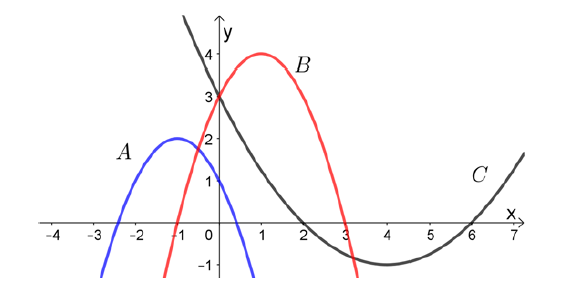
\includegraphics[width=8cm]{Opgave_31-40/Opgave_36/36.png}

Hvilken graf hører til hvilken funktion? Svaret skal begrundes.

\ans

Vi ved at der gælder følgende for en andengradspolynomium. 

Et andengradspolynomie har den generelle forskrift $ax^2 + bx + c$

Fortegnet for a værdien i et andengradspolynomium fortæller om grenene vender opad eller nedad.
Er a positivt $a > 0$ vender grenene opad.
Er a negativt $a < 0$ vender grenene nedad.

Værdien for c i et andengradspolynomium fortæller ved hvilken y værdi andengradspolynomiet skærer y aksen.

Ud fra disse informationer kan vi nu konkludere følgende.

Forskriften $g(x)$ har c værdien $c = 1$ hvilket betyder at $g(x)$ skærer y aksen i $y = 1$ og svarer derfor til det blå andengradspolynomium A
som er den eneste der skærer y aksen i $y = 1$.

Da begge forskrifter $f(x)$ og $h(x)$ skærer y aksen i samme værdi, kigger vi i stedet for på deres a værdier.

Forskriften $f(x)$ har en negativ a værdi $a = -1$ hvilet betyder at grenene på $f(x)$ vender nedad. $f(x)$ svarer derfor til det røde andengradspolynomium
B, hvis grene vender nedad.

Forskriften $h(x)$ har en positiv a værdi $a = \frac{1}{4}$ hvilket betyder at grenene på $h(x)$ vender opad. $h(x)$ svarer derfor til det sorte andengradspolynomium
C, hvis grene vender opad.  